\documentclass[tikz,border=8pt]{standalone}
% Shared look for every TikZ diagram. Load with % Shared look for every TikZ diagram. Load with % Shared look for every TikZ diagram. Load with \input{../../tools/tikz-style.tex}
\usepackage[T1]{fontenc}
\usepackage{lmodern}
\renewcommand{\sfdefault}{lmr}  % diagrams use the same serif as the text
\usetikzlibrary{arrows.meta, positioning, shapes.geometric, calc, fit, backgrounds}
\definecolor{cblue}{HTML}{4C78A8}
\definecolor{corange}{HTML}{F58518}
\definecolor{cgreen}{HTML}{54A24B}
\definecolor{cred}{HTML}{E45756}
\definecolor{cpurple}{HTML}{B279A2}
\definecolor{cgrey}{HTML}{6B6B6B}
\tikzset{
  every picture/.style={font=\sffamily, line width=1.2pt},
  box/.style={draw=#1, fill=#1!12, rounded corners=4pt, align=center, inner sep=7pt, minimum height=1.1cm},
  box/.default=cgrey,
  arrow/.style={-{Stealth[length=3mm]}, draw=cgrey, line width=1.4pt},
  title/.style={font=\sffamily\bfseries\Large},
  note/.style={font=\sffamily\small, text=cgrey, align=center},
}
\AtBeginDocument{\hyphenpenalty=10000 \exhyphenpenalty=10000}

\usepackage[T1]{fontenc}
\usepackage{lmodern}
\renewcommand{\sfdefault}{lmr}  % diagrams use the same serif as the text
\usetikzlibrary{arrows.meta, positioning, shapes.geometric, calc, fit, backgrounds}
\definecolor{cblue}{HTML}{4C78A8}
\definecolor{corange}{HTML}{F58518}
\definecolor{cgreen}{HTML}{54A24B}
\definecolor{cred}{HTML}{E45756}
\definecolor{cpurple}{HTML}{B279A2}
\definecolor{cgrey}{HTML}{6B6B6B}
\tikzset{
  every picture/.style={font=\sffamily, line width=1.2pt},
  box/.style={draw=#1, fill=#1!12, rounded corners=4pt, align=center, inner sep=7pt, minimum height=1.1cm},
  box/.default=cgrey,
  arrow/.style={-{Stealth[length=3mm]}, draw=cgrey, line width=1.4pt},
  title/.style={font=\sffamily\bfseries\Large},
  note/.style={font=\sffamily\small, text=cgrey, align=center},
}
\AtBeginDocument{\hyphenpenalty=10000 \exhyphenpenalty=10000}

\usepackage[T1]{fontenc}
\usepackage{lmodern}
\renewcommand{\sfdefault}{lmr}  % diagrams use the same serif as the text
\usetikzlibrary{arrows.meta, positioning, shapes.geometric, calc, fit, backgrounds}
\definecolor{cblue}{HTML}{4C78A8}
\definecolor{corange}{HTML}{F58518}
\definecolor{cgreen}{HTML}{54A24B}
\definecolor{cred}{HTML}{E45756}
\definecolor{cpurple}{HTML}{B279A2}
\definecolor{cgrey}{HTML}{6B6B6B}
\tikzset{
  every picture/.style={font=\sffamily, line width=1.2pt},
  box/.style={draw=#1, fill=#1!12, rounded corners=4pt, align=center, inner sep=7pt, minimum height=1.1cm},
  box/.default=cgrey,
  arrow/.style={-{Stealth[length=3mm]}, draw=cgrey, line width=1.4pt},
  title/.style={font=\sffamily\bfseries\Large},
  note/.style={font=\sffamily\small, text=cgrey, align=center},
}
\AtBeginDocument{\hyphenpenalty=10000 \exhyphenpenalty=10000}

% Habit 5: subject first (months, purpose lost) versus in context (each algorithm pulls in the topic it needs).
% Algorithm-topic pairs come from the calculus roadmap table in Section 6.
\begin{document}
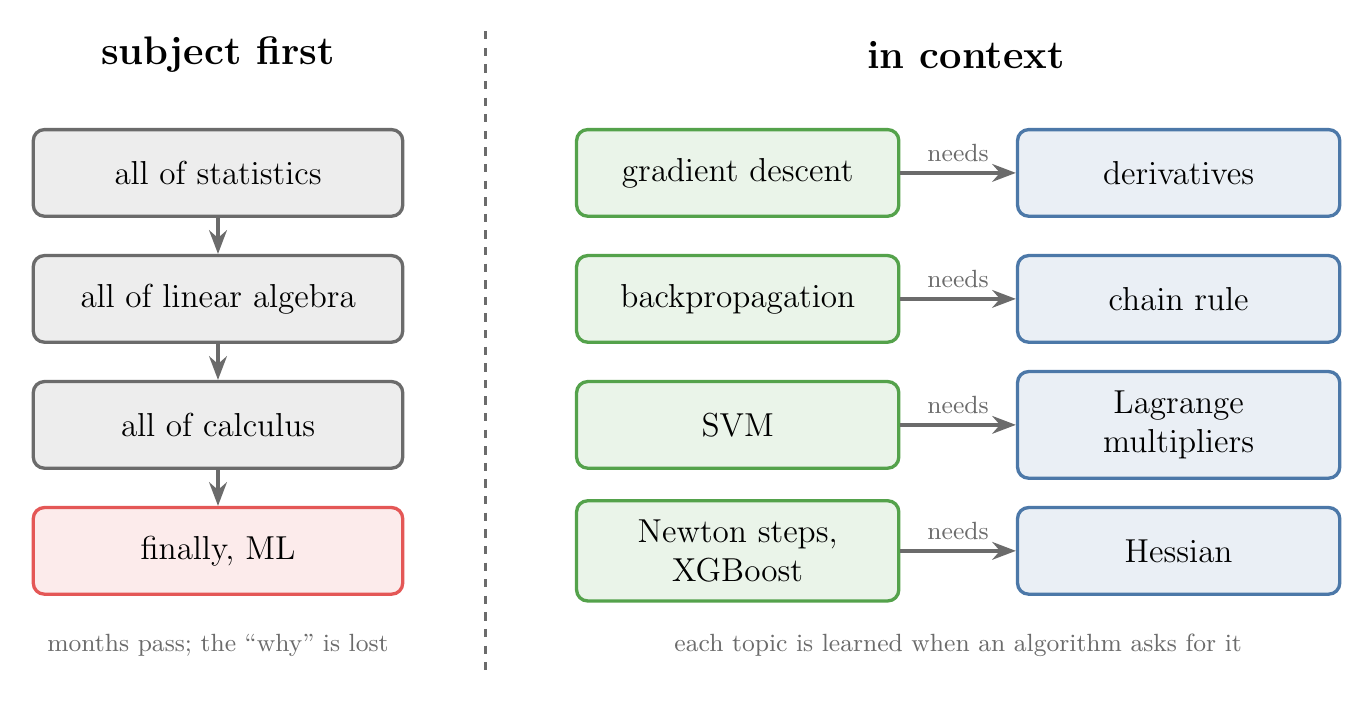
\begin{tikzpicture}[every node/.append style={font=\large}]
  \node[title] at (2, 1.5) {subject first};
  \foreach \i/\t in {0/all of statistics, 1/all of linear algebra, 2/all of calculus} {
    \node[box=cgrey, text width=4.2cm] (s\i) at (2, -1.6*\i) {\t};
  }
  \node[box=cred, text width=4.2cm] (s3) at (2, -4.8) {finally, ML};
  \draw[arrow] (s0) -- (s1); \draw[arrow] (s1) -- (s2); \draw[arrow] (s2) -- (s3);
  \node[note, text width=4.6cm] at (2, -6.0) {months pass; the ``why'' is lost};
  \draw[cgrey, dashed] (5.4, 1.8) -- (5.4, -6.4);
  \node[title] at (11.5, 1.5) {in context};
  \foreach \i/\a/\t in {0/gradient descent/derivatives, 1/backpropagation/chain rule, 2/SVM/Lagrange multipliers, 3/{Newton steps, XGBoost}/Hessian} {
    \node[box=cgreen, text width=3.6cm] (a\i) at (8.6, -1.6*\i) {\a};
    \node[box=cblue, text width=3.6cm] (t\i) at (14.2, -1.6*\i) {\t};
    \draw[arrow] (a\i) -- node[note, above] {needs} (t\i);
  }
  \node[note, text width=8cm] at (11.4, -6.0) {each topic is learned when an algorithm asks for it};
\end{tikzpicture}
\end{document}
